\documentclass[../report.tex]{subfiles}
\begin{document}
\section{Website}
\subsection{Login Screen: index.html}
\begin{figure}[H]
	\centering
	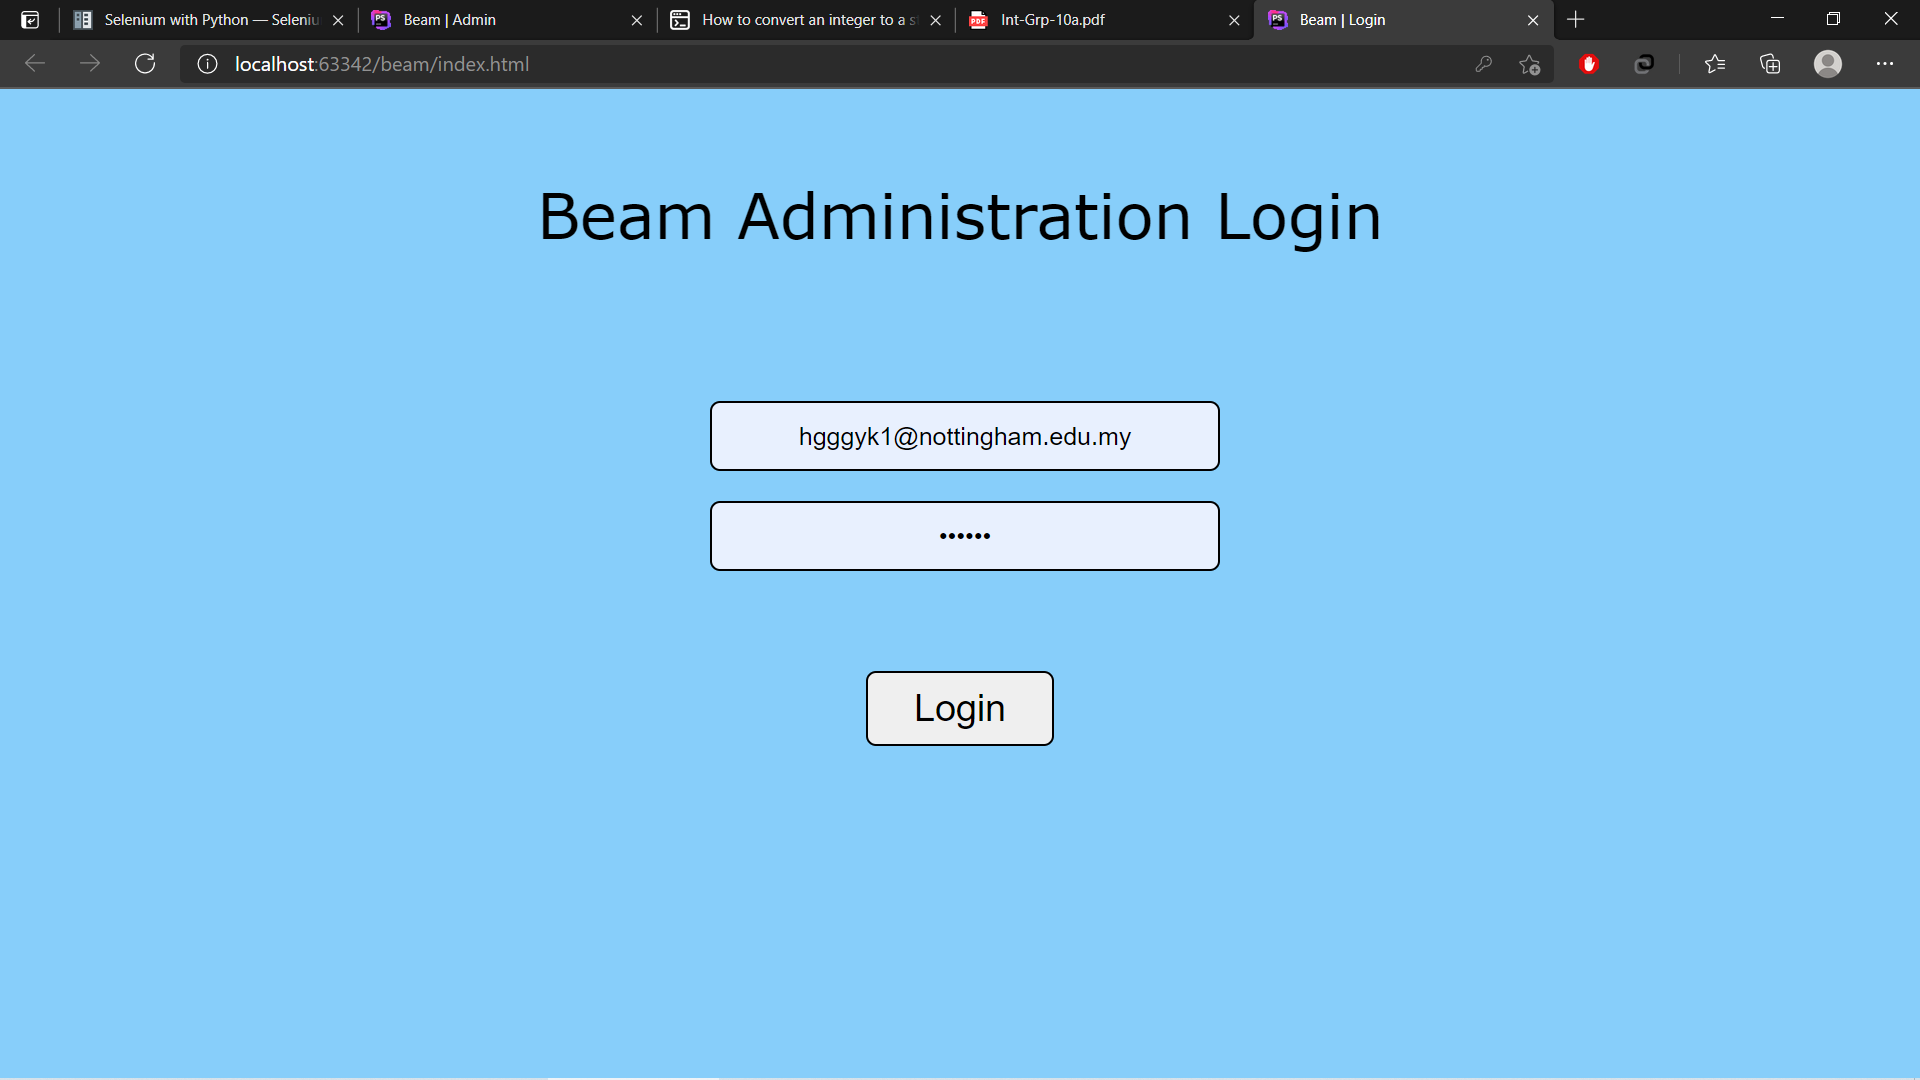
\includegraphics[width=.7\linewidth]{../images/07/01-01-login.png}
	\caption{Login interface of the website}
	\label{fig:07-01-01-login}
\end{figure}

The login interface comprises of a title -- Beam Administration Login, an input field for email, and an input field for password. Upon clicking to the login button, the \textit{login()} function will be executed, as shown below.

\lstinputlisting[language=JavaScript,firstline=36,lastline=50]{../code/web-index.html}

The \textit{login} function takes the email and password entered by the user and sends a promise to Firebase Authentication to check the login credentials. If the credentials are valid, the authentication state will be changed because of a successful user account login and the user will be redirected to \textit{home.html}. The user will remain logged in unless the account is logged out or the user switched to a new tab or window. The state of being logged in will only persist in the current tab or session, and it will be cleared of the tab or window is closed. 

\lstinputlisting[language=JavaScript,firstline=367,lastline=378]{../code/web-home.html}

The \textit{logOut} function logs the user out from the account and redirects the user back to the login page. If the user accesses the home page without going through the login page, the system will check if the user has logged in on Firebase Authentication. If not, the user will be redirected to the login page. The user will remain on the home page if Firebase Authentication detects that the user has performed a successful login.

\subsection{Home Screen: home.html}
\subsubsection{Home Component}
\begin{figure}[H]
	\centering
	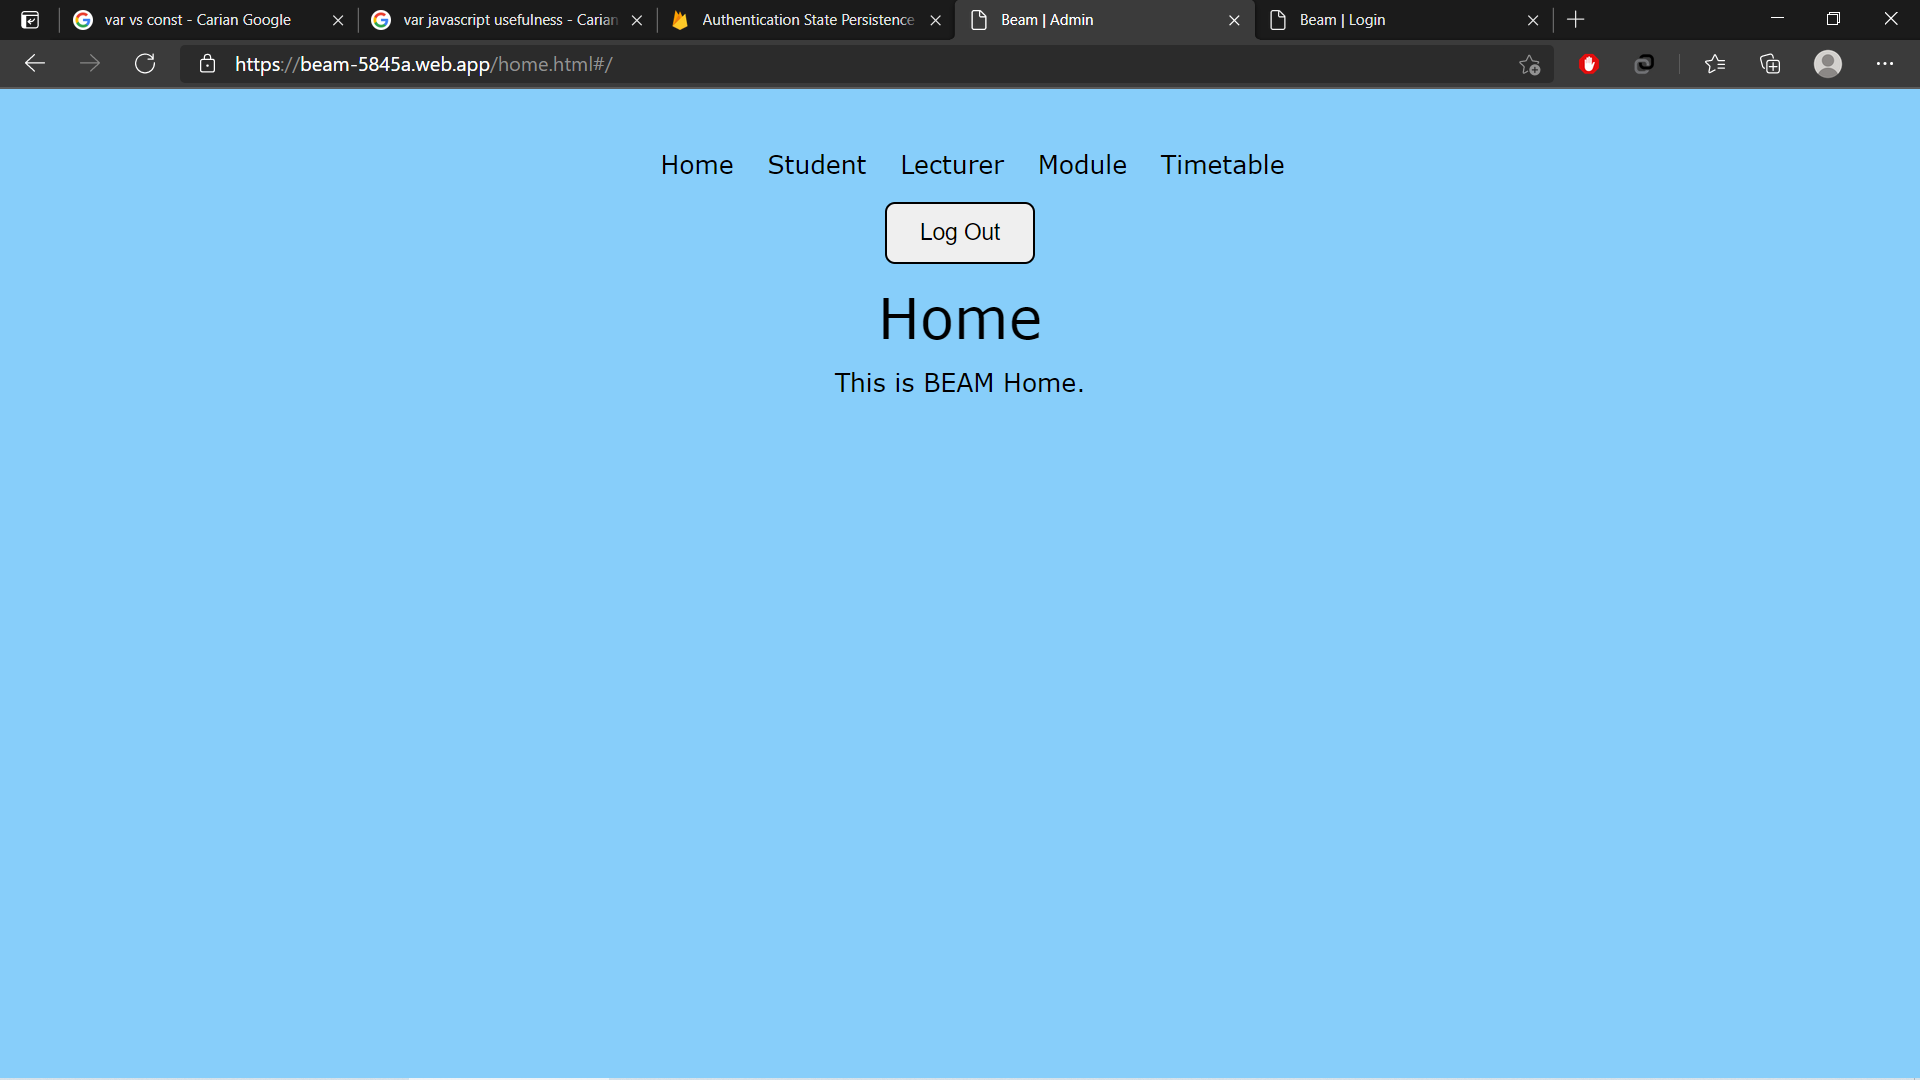
\includegraphics[width=.7\linewidth]{../images/07/01-02-home.png}
	\caption{This is the Home interface of the website. Note that it changed to any important announcement from the university}
	\label{fig:07-01-02-home}
\end{figure}

\lstinputlisting[language=JavaScript,firstline=86,lastline=105]{../code/web-home.html}

This home page is a \textit{single-page application (SPA)} that contains all the features needed for the admin to enter data into the database. Vue.js functions are imported using CDN and used to enable us to build a \textit{SPA}. This Vue.js \textit{SPA} is created in a \textit{$<$div$>$} with an id of \textit{app} with a \textit{router} to link each tab of the navigation with a path. The router will load the contents of each tab in \textit{hash} mode, which means \# is used before the navigation path is passed internally. Since this section of the URL is not sent to the server, no special treatment is required on the server level.
 
The code above directs each path to a component. Every component is an x-template, where the html elements (front-end) of a template in stored in a \textit{$<$script$>$} tag in a HTML file. The router will redirect the tabs to their respective template.

\medskip
\subsubsection{Student Component}
\begin{figure}[H]
	\centering
	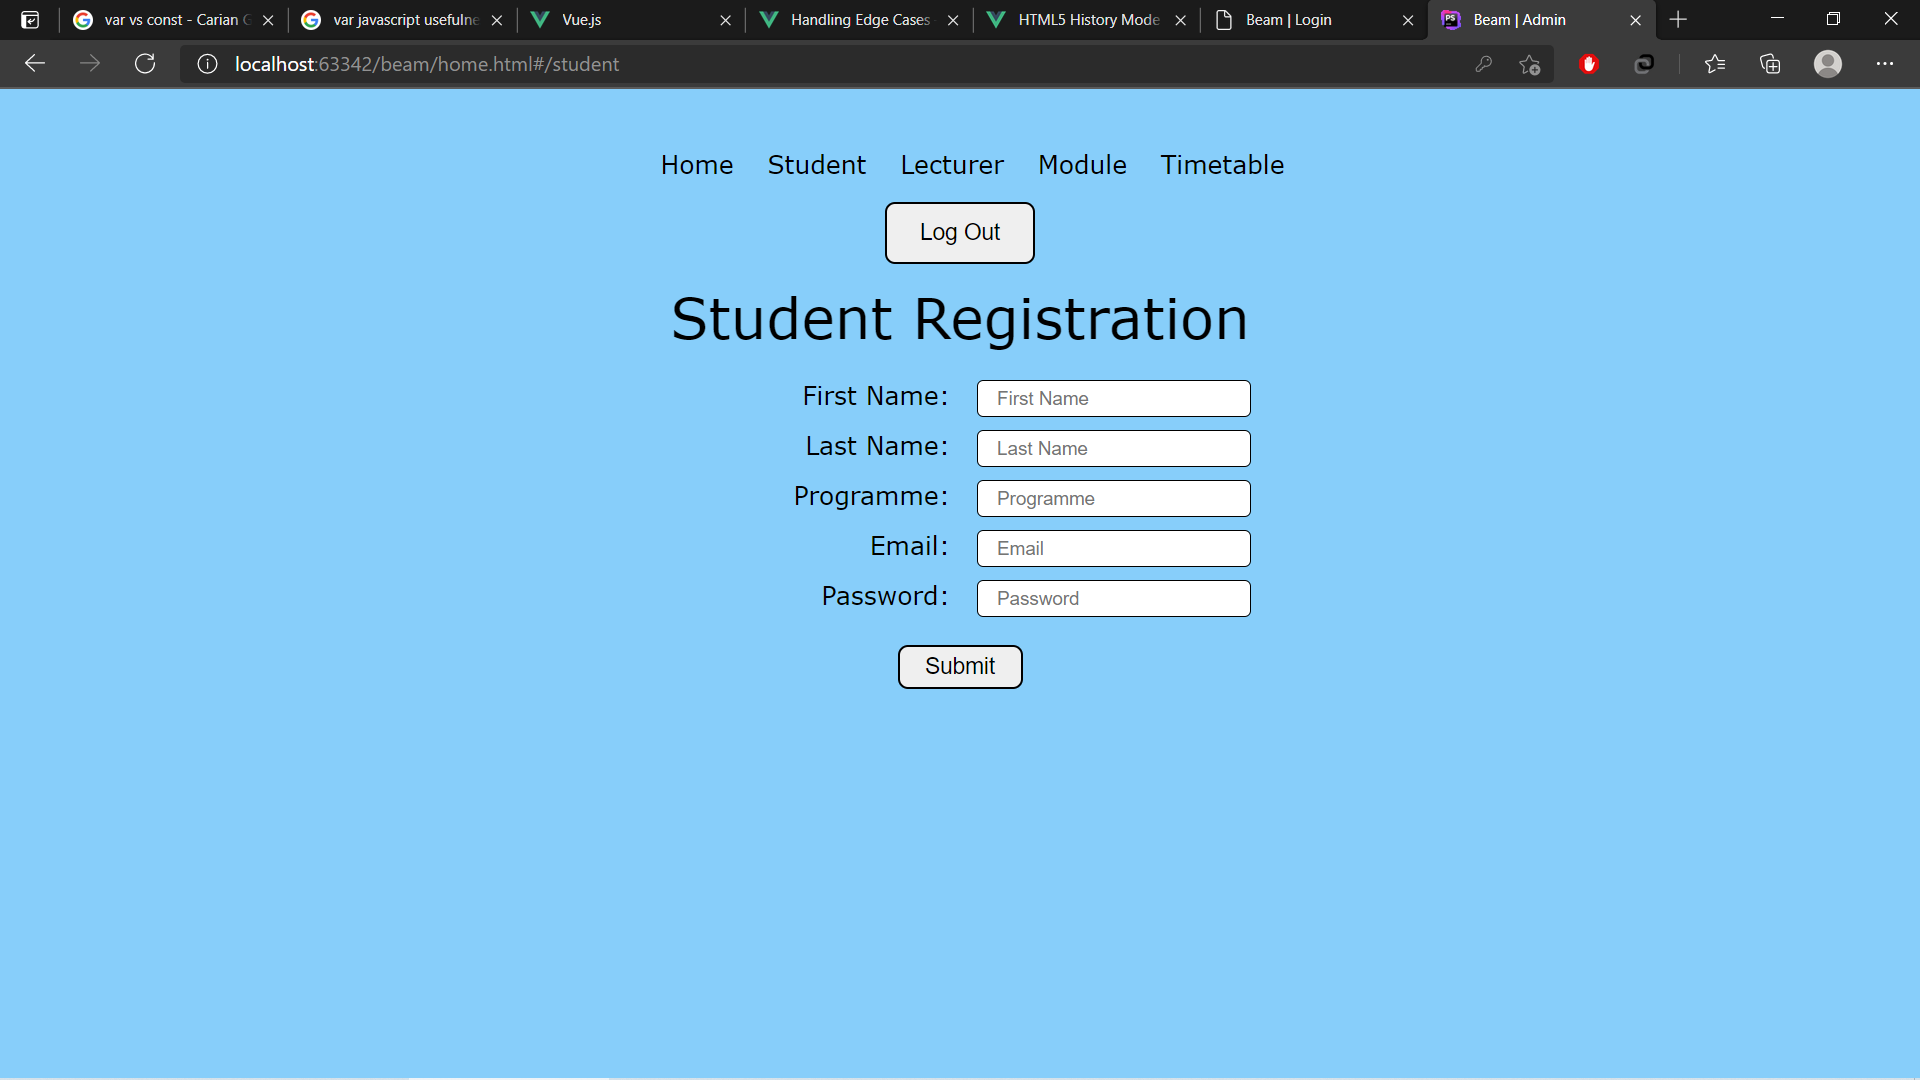
\includegraphics[width=.7\linewidth]{../images/07/01-03-student-reg.png}
	\caption{This is the Student Registration interface of the website}
	\label{fig:07-01-03-student}
\end{figure}

\lstinputlisting[language=JavaScript,firstline=144,lastline=166]{../code/web-home.html}

When the \textit{email} and \textit{password} are sent to Firebase Authentication to create a new account for the student, the \textit{first name}, \textit{last name}, \textit{programme}, and \textit{email}, are entered under the \textit{student} node and grouped by the student account’s \textit{user uid}. Under the \textit{users} node, the role of the account (Student) and the \textit{programme} are entered, grouped by \textit{user uid}. With the programme name, the system will fetch all the \textit{module ids} of the core modules of the \textit{programme} and store them in the \textit{modules} node under \textit{user uid} node, which is also under \textit{users} node. The system will also register the \textit{user uid} of the students under \textit{students} node of each \textit{modules} node.

\medskip
\subsubsection{Lecturer Component}
\begin{figure}[H]
	\centering
	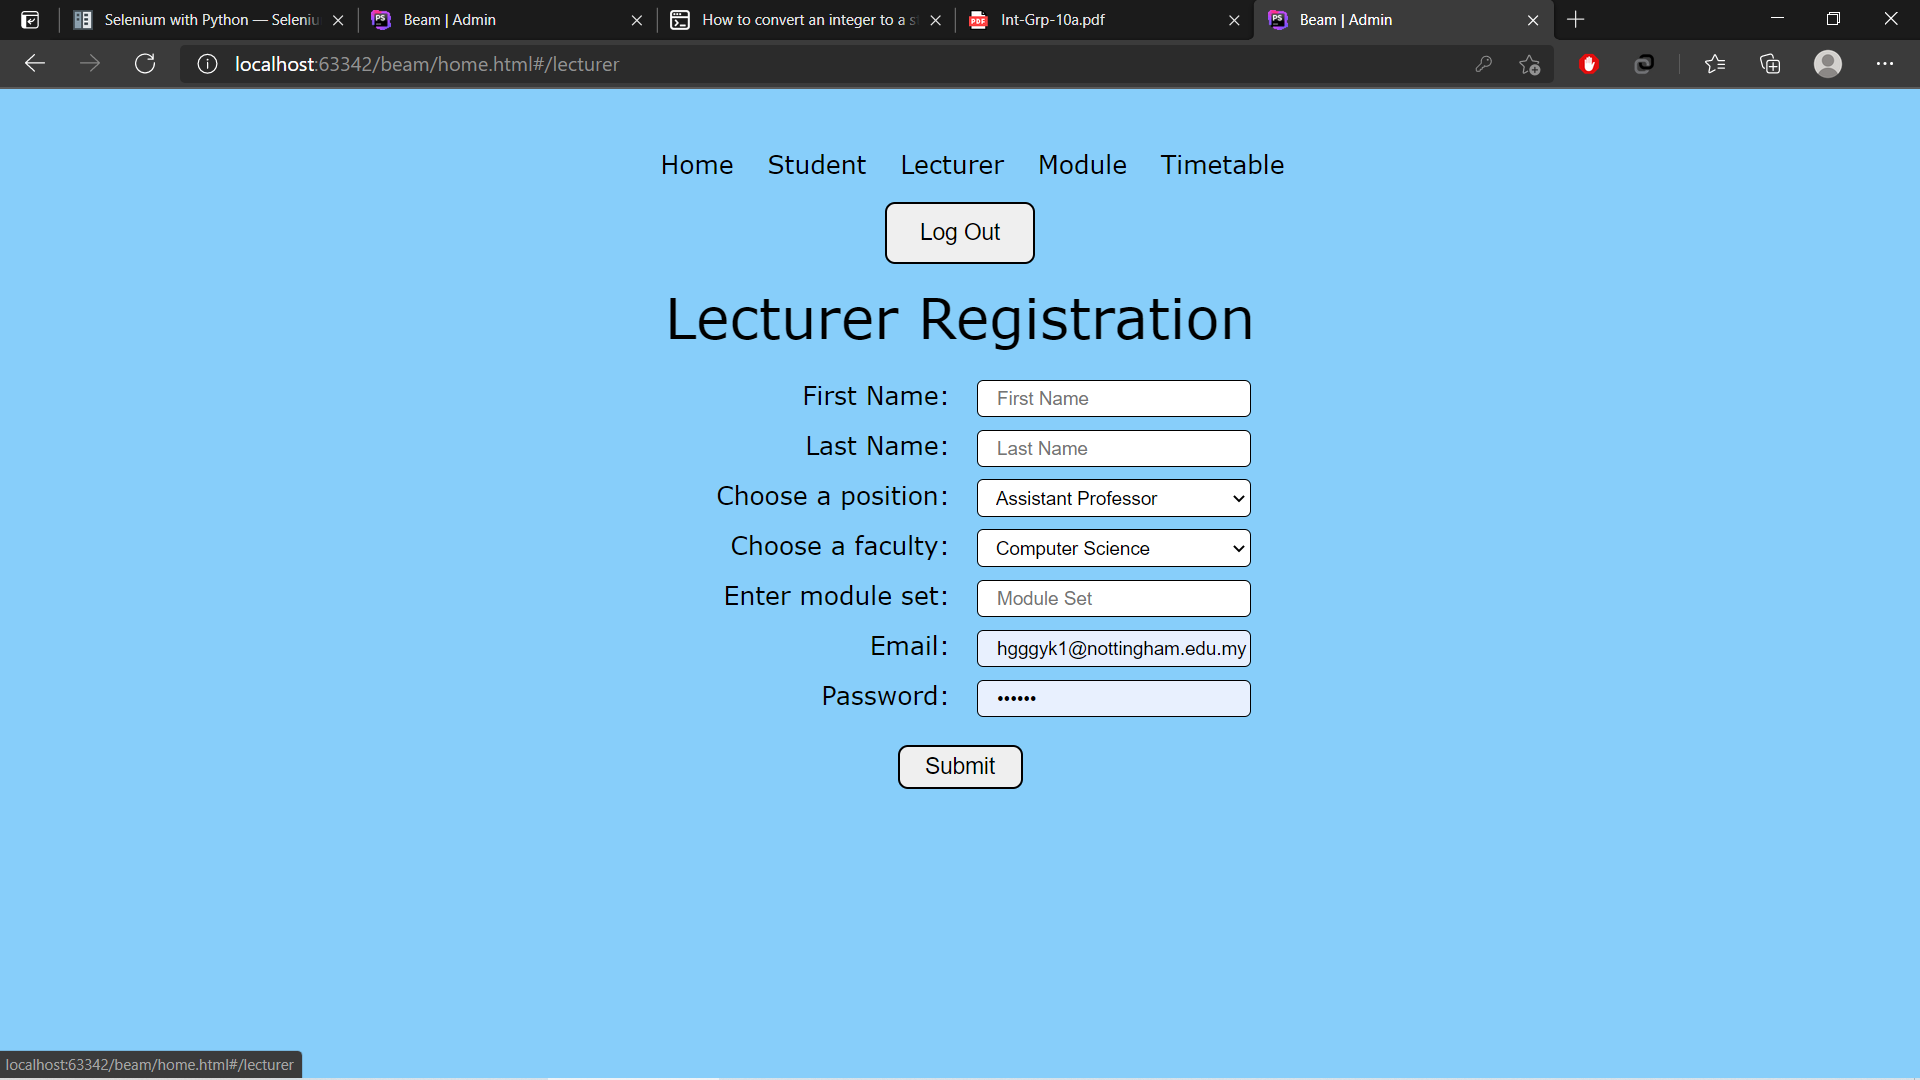
\includegraphics[width=.7\linewidth]{../images/07/01-04-lecturer-reg.png}
	\caption{This is the Lecturer Registration interface of the website}
	\label{fig:07-01-04-lecturer}
\end{figure}

\lstinputlisting[language=JavaScript,firstline=217,lastline=241]{../code/web-home.html}

When the \textit{email} and \textit{password} are sent to Firebase Authentication to create a new account for the lecturer, the \textit{first name}, \textit{last name}, \textit{position}, \textit{faculty} and \textit{email}, are entered under the \textit{lecturer} node and grouped by the lecturer account’s \textit{user uid}. Under the \textit{users} node, the role of the account (Lecturer), module set and the \textit{programme} are entered, grouped by \textit{user uid}. With the programme name, the system will fetch all the \textit{module ids} of the modules under the module \textit{set} selected and store them in the \textit{modules} node under \textit{user uid} node, which is also under \textit{users} node. The system will also register the user uid of the lecturers under \textit{lecturers} node of each \textit{modules} node.

\medskip
\subsubsection{Module Component}
\begin{figure}[H]
	\centering
	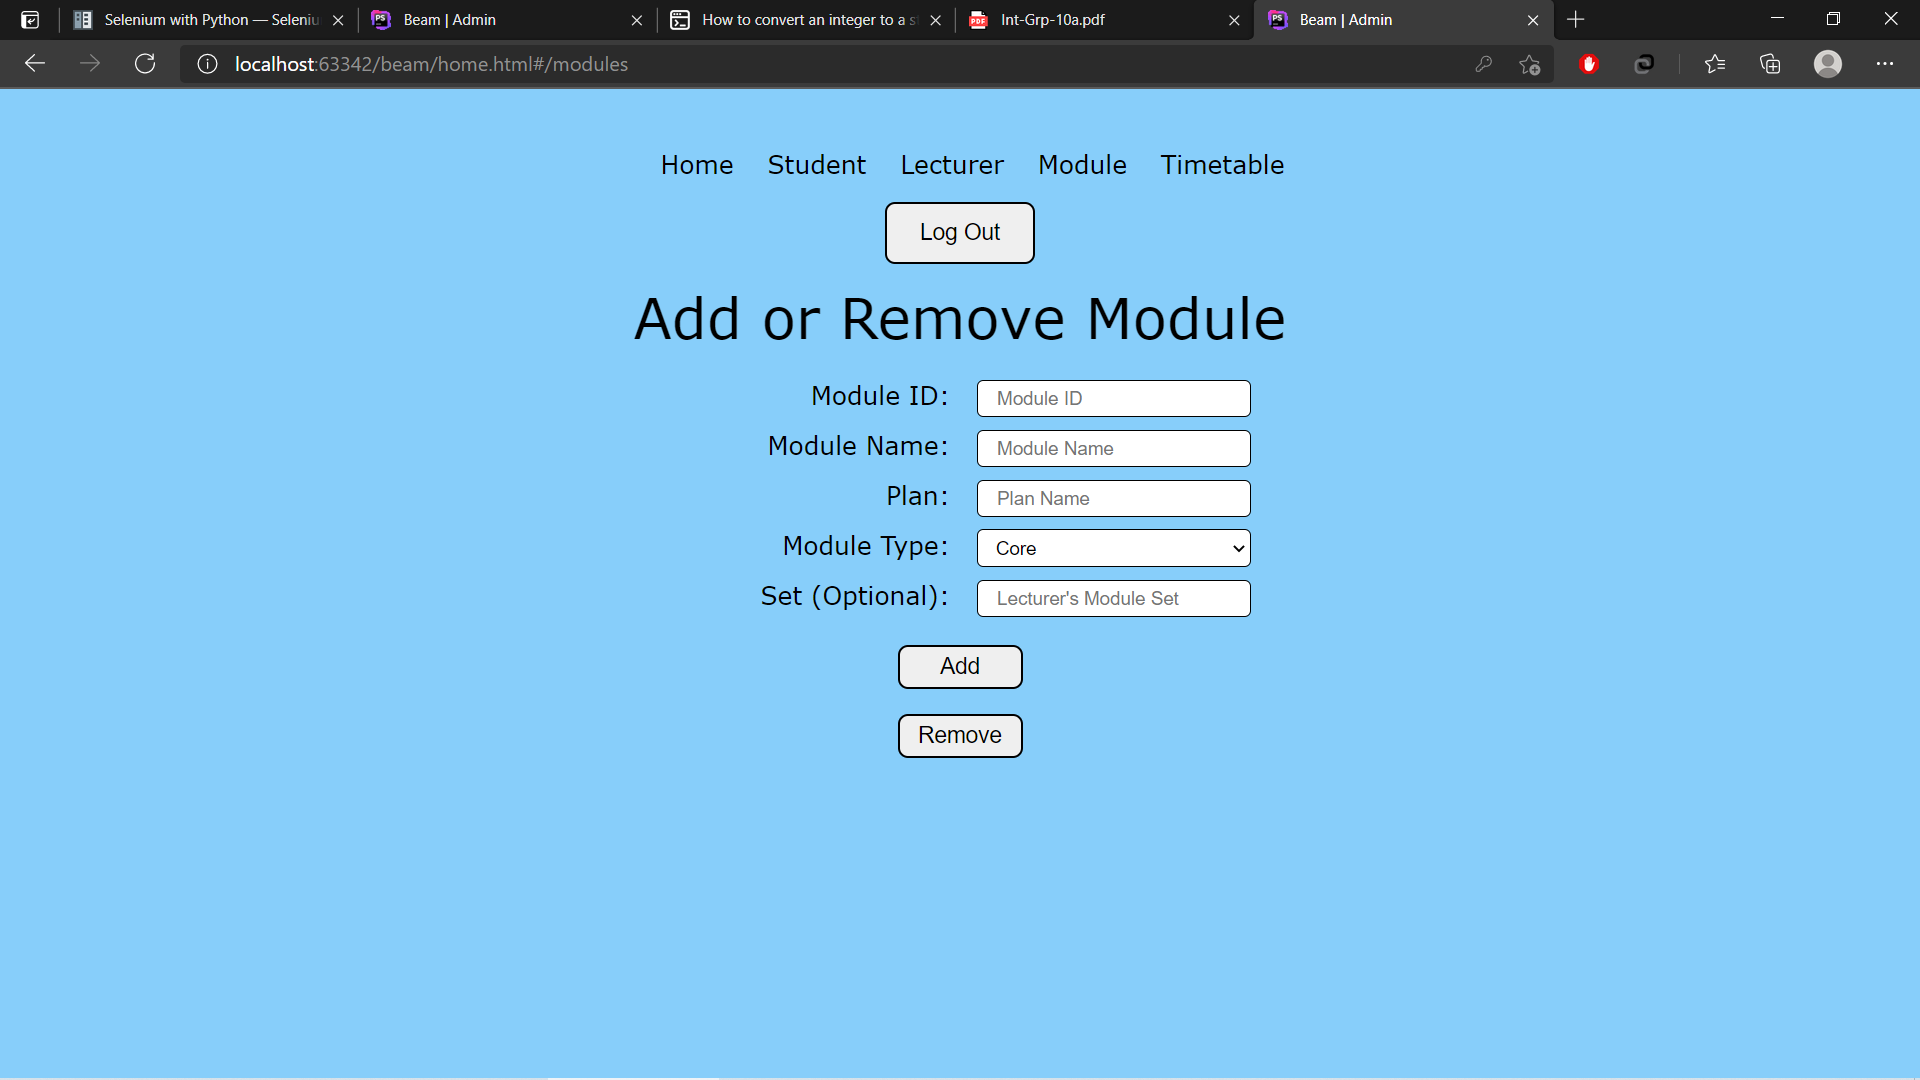
\includegraphics[width=.7\linewidth]{../images/07/01-05-module.png}
	\caption{This is the Add or Remove Module interface of the website}
	\label{fig:07-01-05-module}
\end{figure}

\lstinputlisting[language=JavaScript,firstline=276,lastline=299]{../code/web-home.html}

To add module details to the database, the system will enter the \textit{module names} under the \textit{module id}, which is under the \textit{modules} node. By the names of the \textit{academic plan} which the \textit{modules} fall under, the \textit{modules ids} of these \textit{modules}, grouped by \textit{module type}, will be placed under the \textit{plan name}, which is under the \textit{plan} node. For the modules taught by a lecturer, the \textit{module ids} will be stored under \textit{module set}, under the modules' \textit{plan name}, which is also under the \textit{plan} node.

\lstinputlisting[language=JavaScript,firstline=300,lastline=311]{../code/web-home.html}

To delete module details from the database, fetch the \textit{module id} from the website and query the modules and remove the data under the matched \textit{module id}. The system can remove the same module ids from the database directory: \textit{plan/plan name/module type}. 

\medskip
\subsubsection{Timetable Component}
\begin{figure}[H]
	\centering
	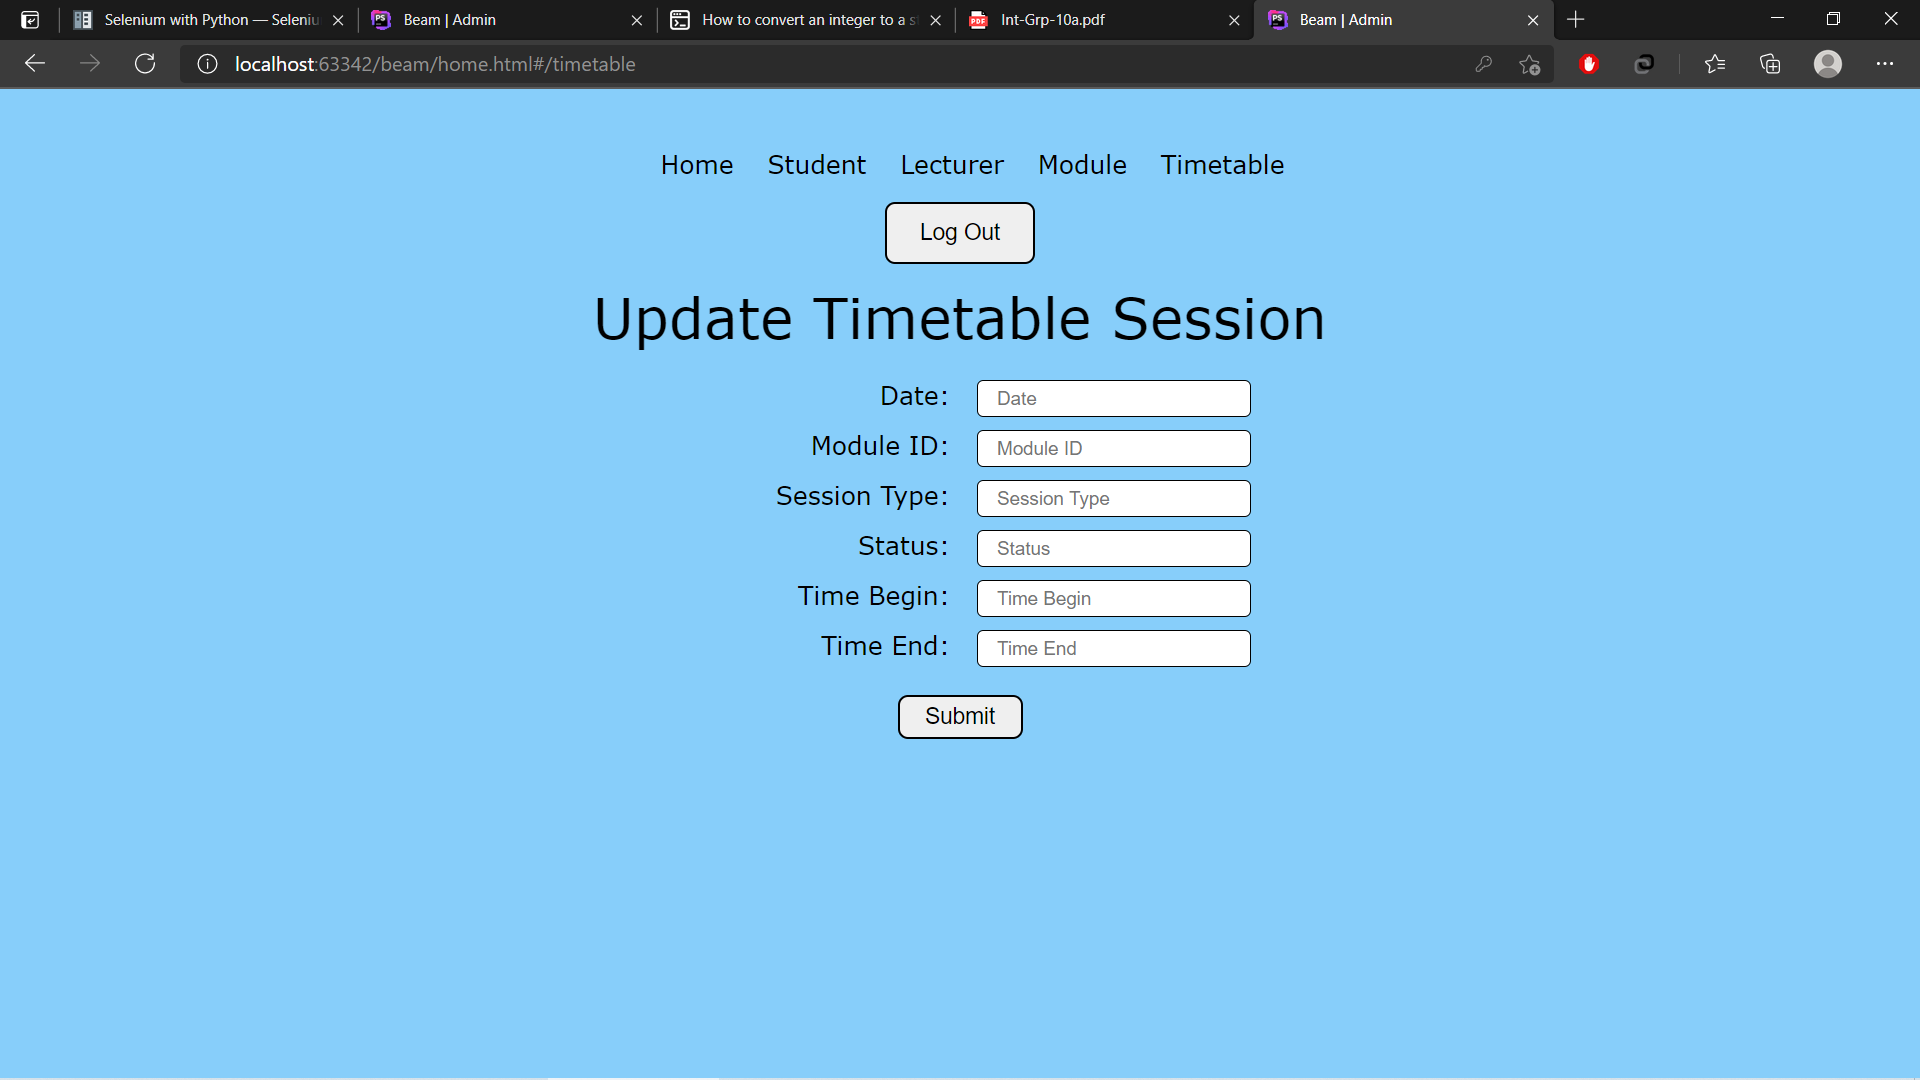
\includegraphics[width=.7\linewidth]{../images/07/01-06-timetable.png}
	\caption{This is the Update Timetable Session interface of the website}
	\label{fig:07-01-06-timetable}
\end{figure}

\lstinputlisting[language=JavaScript,firstline=334,lastline=356]{../code/web-home.html}

The system sends the \textit{date}, \textit{module\_id}, \textit{session type}, \textit{session status} (Opened/Closed), \textit{time\_begin}, and \textit{time\_end} to the database. Under the \textit{timetable} node, the module details will be entered, grouped by the \textit{date}. Under the \textit{modules\_session} node, the module details will be entered, grouped by the \textit{module\_id}. This groups the sessions of a module under a \textit{module\_id}.

\medskip
\subsection{Test Results}
The changes reflected in the database due to the Python script will be shown below in screenshots
\begin{figure}[H]
	\centering
	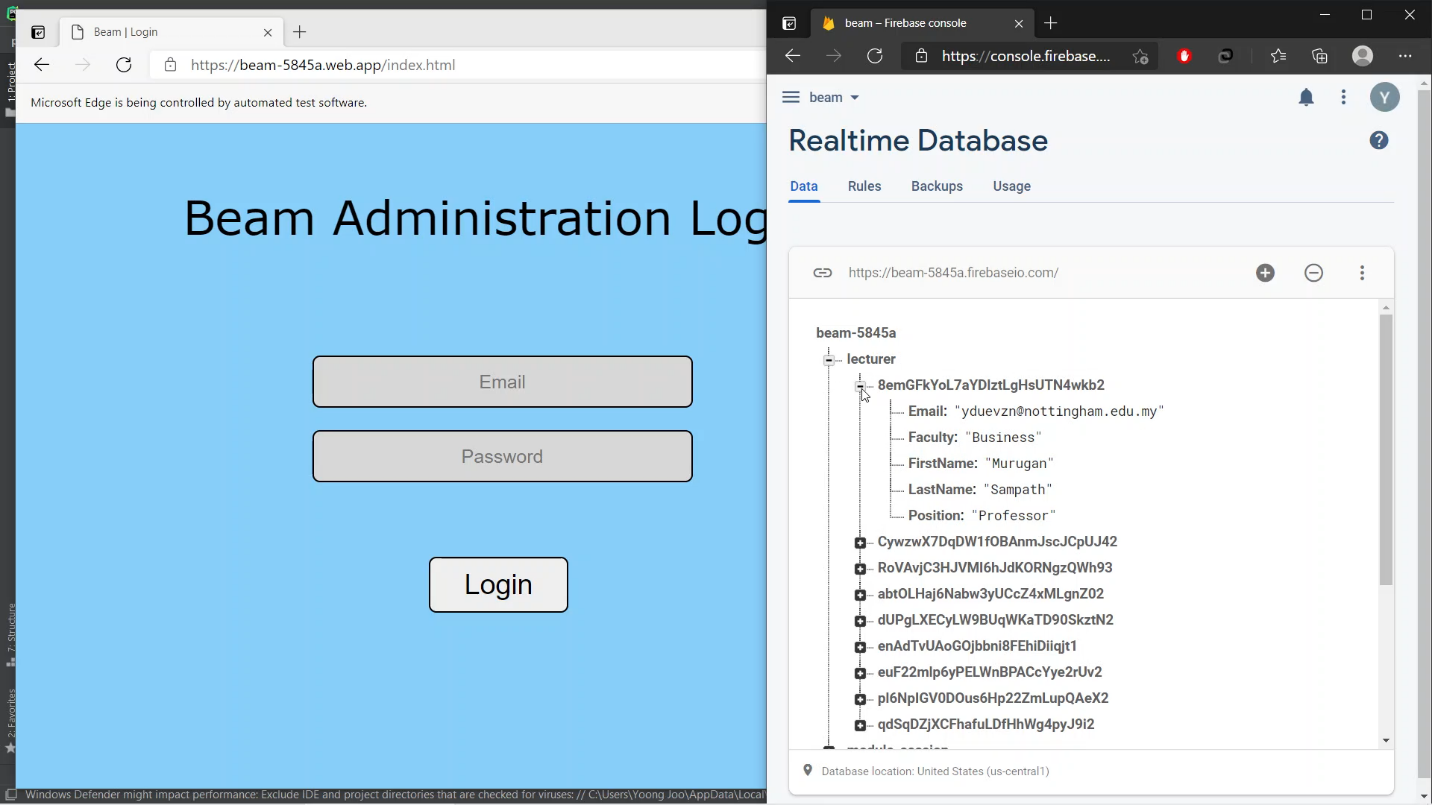
\includegraphics[width=.7\linewidth]{../images/07/01-07-test-lecturer.png}
	\caption{Changes made to the lecturer node}
	\label{fig:07-01-07-test-lecturer}
\end{figure}
\begin{figure}[H]
	\centering
	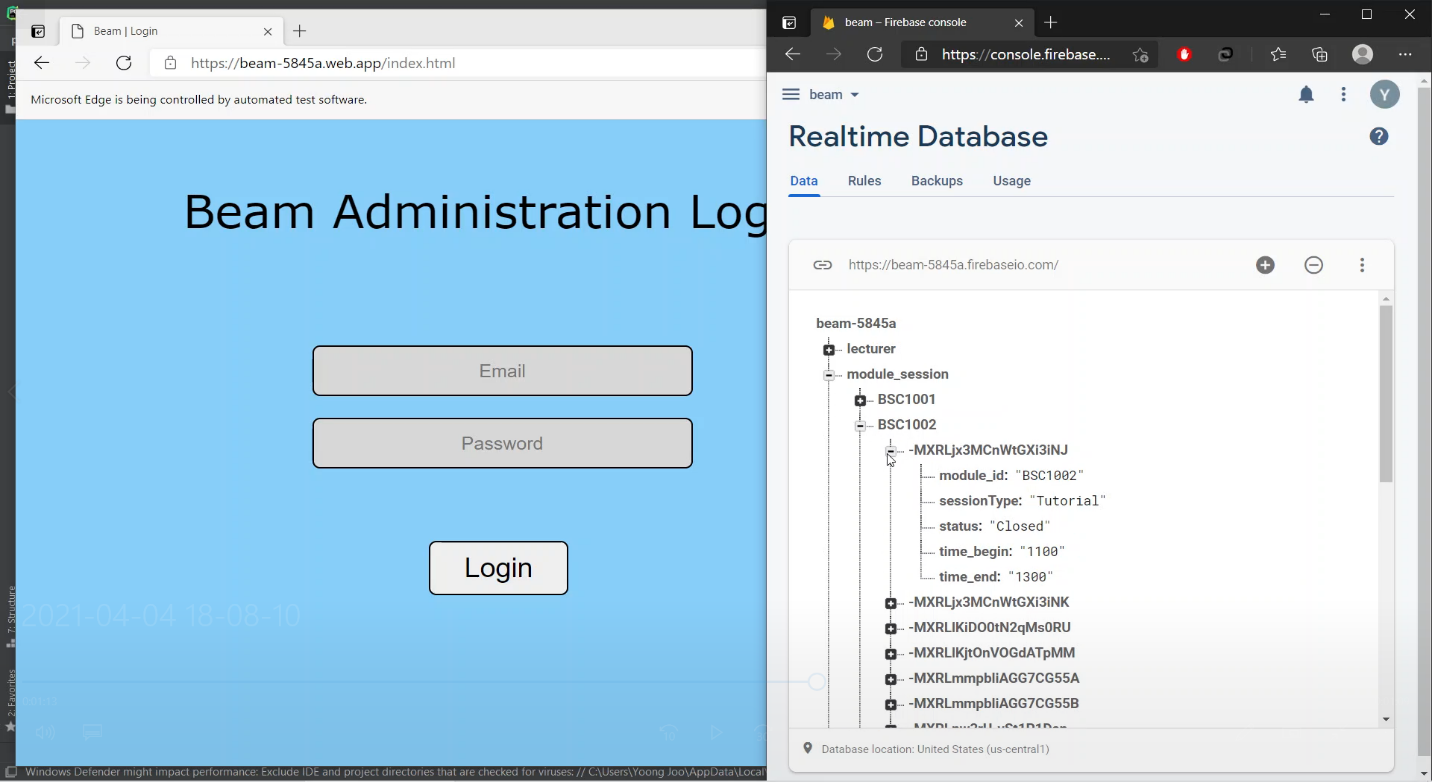
\includegraphics[width=.7\linewidth]{../images/07/01-08-test-module-session.png}
	\caption{Changes made to the module\_session node}
	\label{fig:07-01-08-test-module-session}
\end{figure}
\begin{figure}[H]
	\centering
	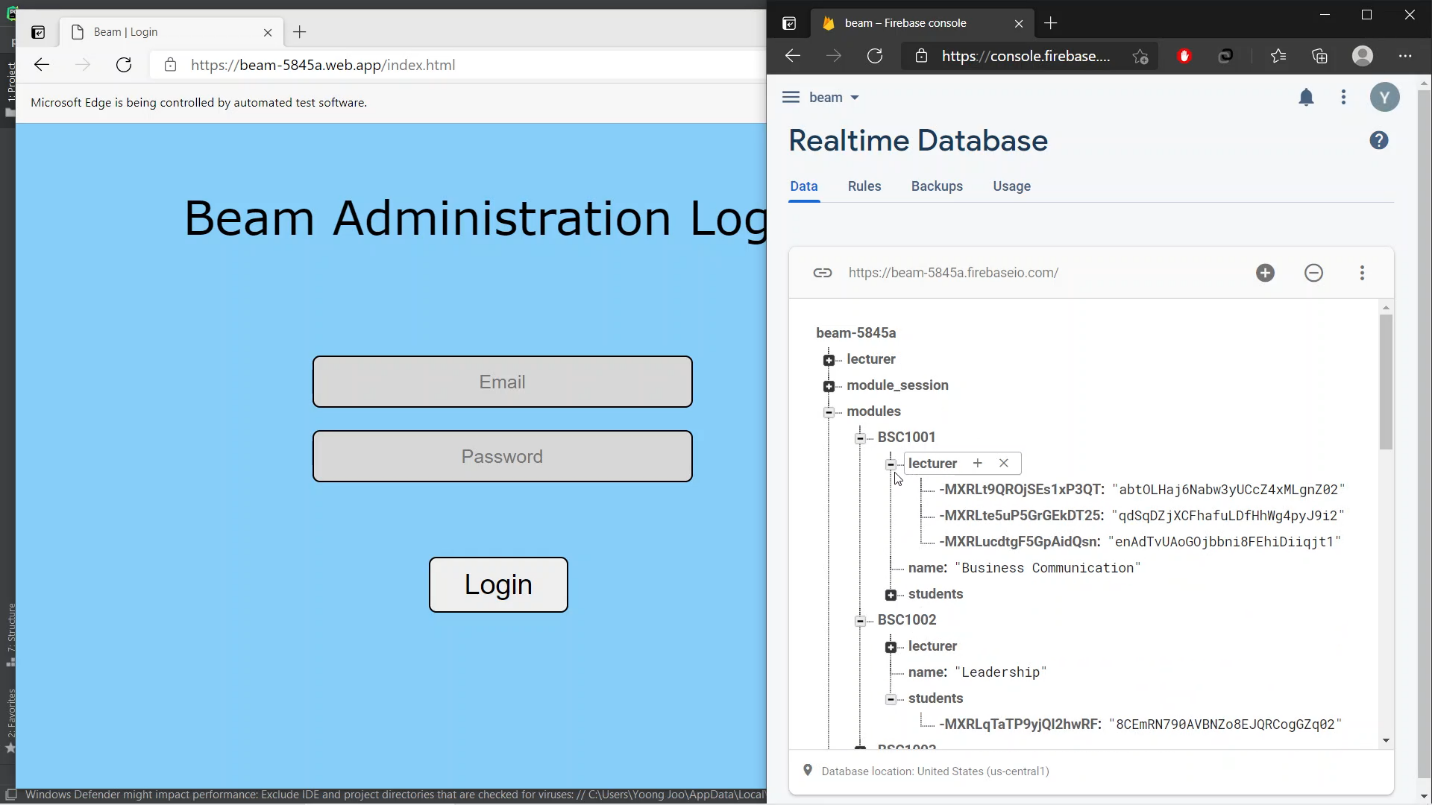
\includegraphics[width=.7\linewidth]{../images/07/01-09-test-module.png}
	\caption{Changes made to the modules node}
	\label{fig:07-01-09-test-module}
\end{figure}
\begin{figure}[H]
	\centering
	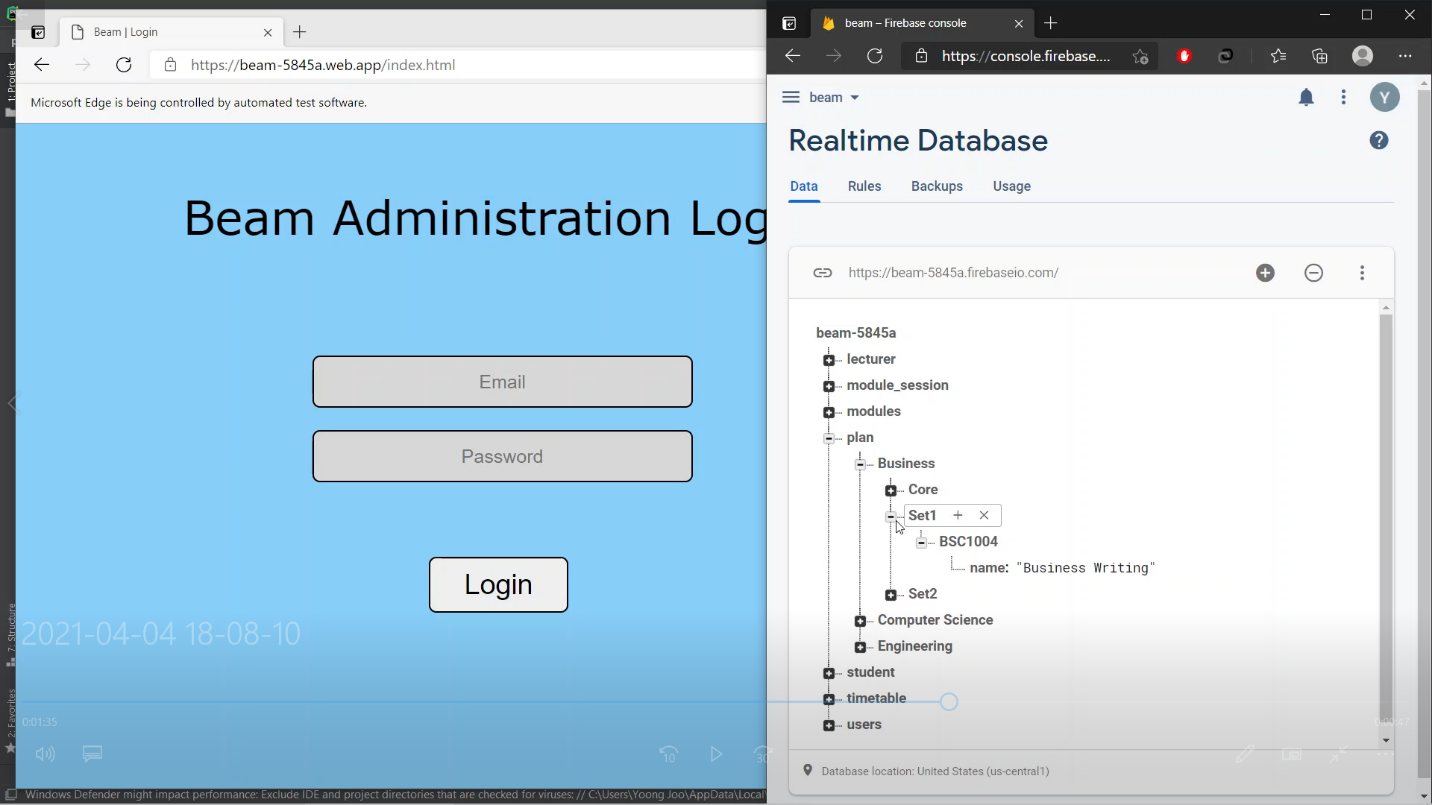
\includegraphics[width=.7\linewidth]{../images/07/01-10-test-plan.png}
	\caption{Changes made to the plan node}
	\label{fig:07-01-10-test-plan}
\end{figure}
\begin{figure}[H]
	\centering
	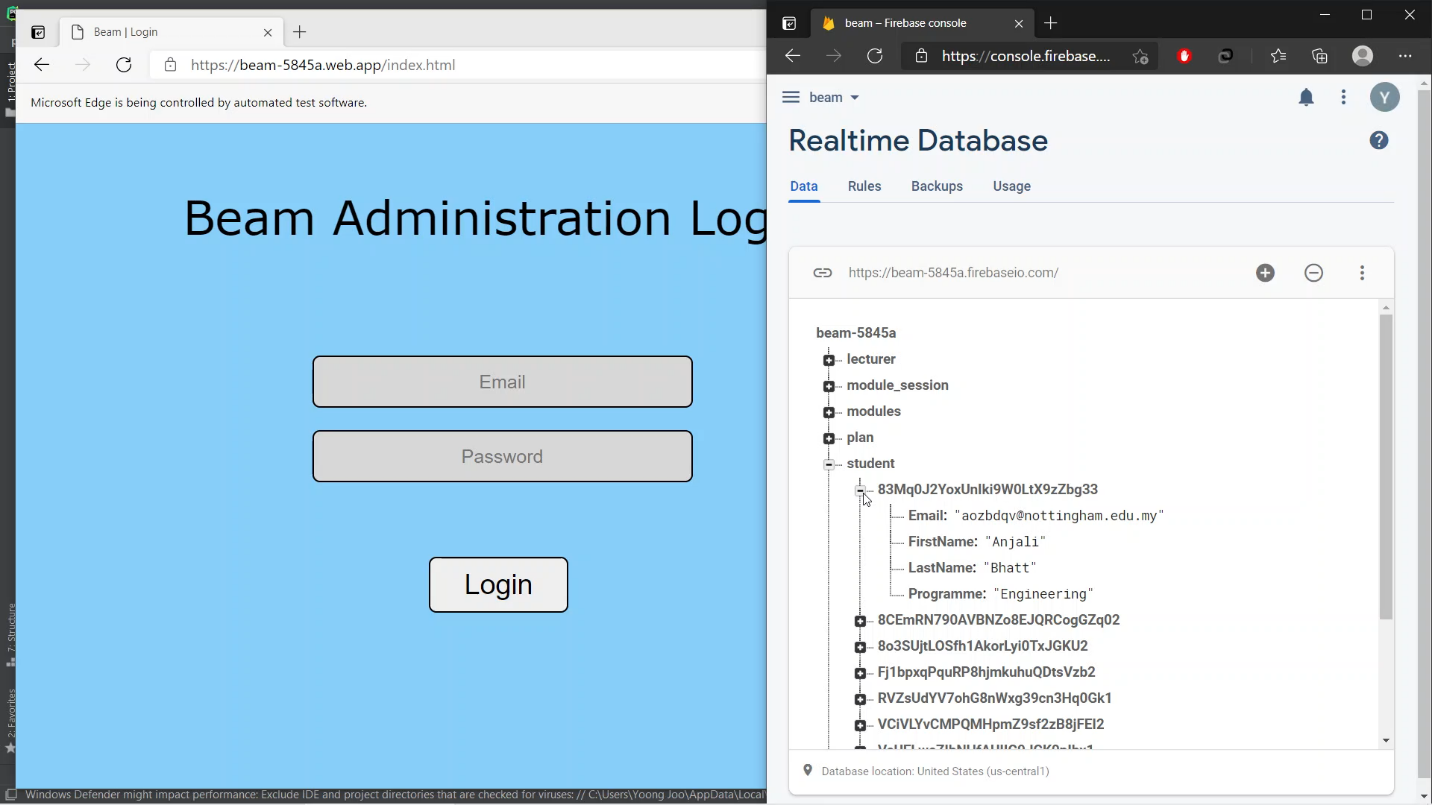
\includegraphics[width=.7\linewidth]{../images/07/01-11-test-student.png}
	\caption{Changes made to the student node}
	\label{fig:07-01-11-test-student}
\end{figure}
\begin{figure}[H]
	\centering
	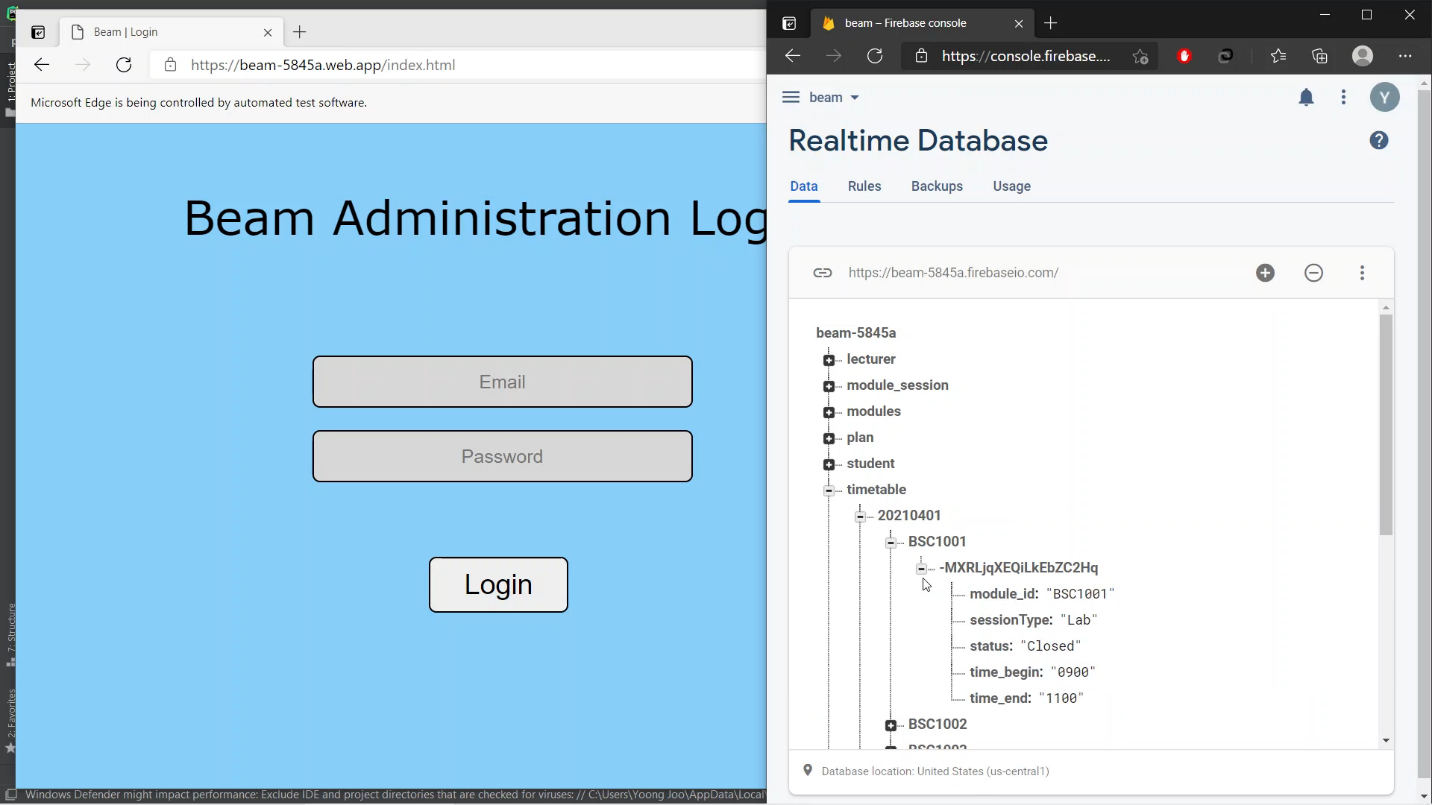
\includegraphics[width=.7\linewidth]{../images/07/01-12-test-timetable.png}
	\caption{Changes made to the timetable node}
	\label{fig:07-01-12-test-timetable}
\end{figure}
\begin{figure}[H]
	\centering
	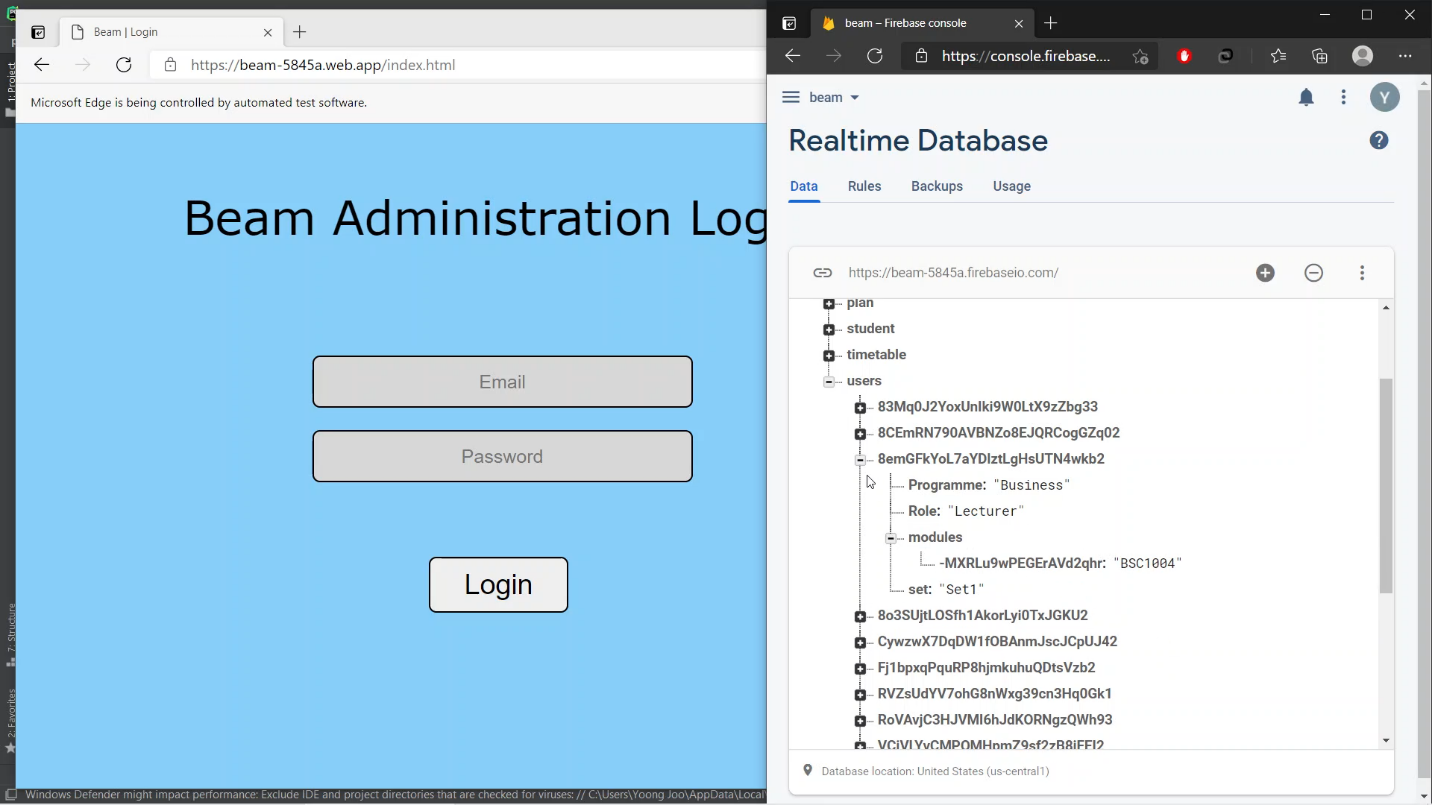
\includegraphics[width=.7\linewidth]{../images/07/01-13-test-users.png}
	\caption{Changes made to the users node}
	\label{fig:07-01-13-test-users}
\end{figure}

\section{Application}
\subsection{Overview of Classes}

\subsection{Splash Screen}

\subsection{Login Screen}

\subsection{Home Screen}

\subsection{Settings Screen}

\subsection{Data Fetching Classes}

\subsection{BLE Services and Related Classes}

\subsection{Test Results}
\end{document}